\section{Conclusiones}
\begin{frame}
	\frametitle{Conclusiones}
	\begin{figure}
	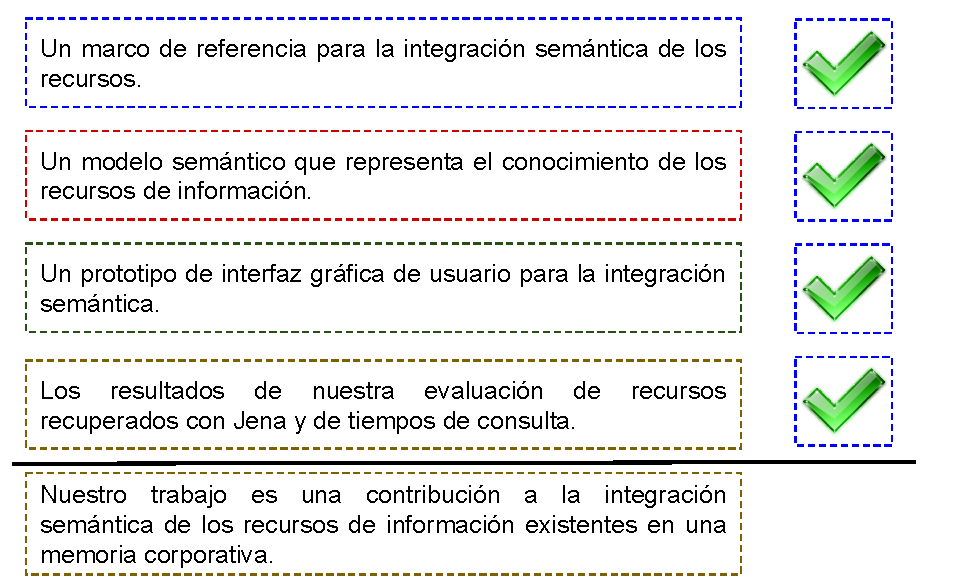
\includegraphics[scale=0.6]{ConclusionesObj} 
	\end{figure}
\end{frame}

\begin{frame}
	\frametitle{Conclusiones}
	\begin{exampleblock}{Hip�tesis}
	\justifying 
	\textbf{El uso de las \textit{tecnolog�as sem�nticas} es adecuado para lograr la \textit{integraci�n sem�ntica} de \textit{recursos de informaci�n} en una \textit{memoria corporativa}}.
	\end{exampleblock}
	
	\begin{block}{Ventajas de las Tecnolog�as Sem�nticas}
	\begin{itemize}
	\item \justifying Formato est�ndar.
	\item \justifying Modelos flexibles, extensibles y reutilizables.
	\item \justifying Lenguajes est�ndar.
	\item \justifying Modelos con conocimiento expl�cito e impl�cito.
	\item \justifying Inferencia para materializar tripletas RDF.
	\item \justifying Aplicaciones gen�ricas.
	\end{itemize}
	\end{block}
\end{frame}

\begin{frame}
	\frametitle{Recomendaciones}

\end{frame}